\chapter{Modyfikacja algorytmu NPQGA}
\label{cha:modyfikacja}
Przestawiony w poprzednim rozdziale algorytm NPQGA nadaje się do rozwiązywania problemu przydziału kwadratowego, lecz w kontekście stworzenia aplikacji, będącej jednym z celów niniejszej pracy, zostały wprowadzone liczne modyfikacje, a także algorytm został uzupełniony o dodatkowe, nie zaproponowane przez jego autorów, cechy. Wszystkie opisane zmiany, a także dodane funkcjonalności zostały zaproponowane i uzgodnione z opiekunem pracy i zostaną przedstawione w tym rozdziale. Jednakże, główna cecha algorytmu, jaką jest wykorzystanie bitów kwantowych do reprezentacji rozwiązań problemu, pozostała bez zmian. Kodowanie osobników wygląda tak samo, jak zostało to opisane w rozdziale poprzednim.

\section{Lista zmian i modyfikacji}
\subsection{Nierównoległa wersja algorytmu}
Główną zmianą wprowadzoną do implementowanego algorytmu jest zrezygnowanie z równoległej wersji algorytmu. Istnieje zatem tylko jedna populacja, która ewoluuje razem z kolejnymi iteracjami algorytmu. Implikuje to również brak potrzeby wymiany informacji pomiędzy uniwersami, a także pomiędzy populacjami w każdym z uniwersów.

\subsection{Operator katastrofy}
W związku z rezygnacją z wielu populacji rozwijanych równolegle, zaniechano również korzystania z operatora katastrofy. Jego stosowanie mogłoby powodować utratę wypracowanego z czasem dobrego rozwiązania, jeśli to nie zmieniałoby się od ustalonej liczby pokoleń. W przypadku wielu równolegle ewoluujących populacji, użycie tego operatora mogłoby pozwolić na wyjście z lokalnego minimum w danej populacji, lecz w przypadku jednej, powodowałoby to utratę jedynego znalezionego rozwiązania i rozpoczęcie szukania optimum od początku. W sytuacji, gdy operator zostałby użyty pod koniec wykonywania algorytmu, szukane od nowa rozwiązanie, w związku z małą liczbą pozostałych iteracji, mogłoby odbiegać bardzo od faktycznego optimum.

\subsection{Operatory selekcji}
W zmodyfikowanej wersji algorytmu zostały wykorzystane dwie wersje operatora selekcji. Pierwsza z nich polega na selekcji ruletkowej. Funkcja dopasowania rozwiązań została uzyskana z funkcji celu w następujący sposób:
\newline
\begin{equation}
f(x_i)= F_{c max} - F(x_i)
\end{equation}
\newline
gdzie $f(x_i)$ jest funkcją dopasowania \textit{i-tego} rozwiązania w pokoleniu, $F_{c max}$ jest wartością funkcji celu dla najgorszego rozwiązania w danym pokoleniu, czyli o największym koszcie przydziału, a $F(x_i)$ jest funkcją celu \textit{i-tego} rozwiązania w pokoleniu. W ten sposób funkcja dopasowania jest zawsze nieujemna, a większa jej wartość oznacza, że rozwiązanie ma lepsze dopasowanie. Następnie w oparciu o wartości dopasowania rozwiązań, w standardowy sposób, budowane jest koło ruletki.

Drugim z operatorów jest operator selekcji bazujący na rankingu rozwiązań. Rozwiązania w aktualnym pokoleniu są szeregowane rosnąco według wartości funkcji celu, czyli rozwiązania o mniejszej wartości funkcji celu mają niższy indeks na liście, czyli mają w rankingu wyższe miejsce. Następnie w oparciu o ranking budowana jest funkcja, której wartość określa prawdopodobieństwo wyboru danego rozwiązania podczas selekcji. Istnieje wiele wariantów tych funkcji. W zaimplementowanym operatorze selekcji rankingowej wykorzystano funkcję liniową o poniższym wzorze na prawdopodobieństwo wyboru rozwiązania na \textit{i-tej} pozycji w rankingu:
\newline
\begin{equation}
p_s(x_i)=\frac{1}{n}(\eta_{max}-(\eta_{max}-\eta_{min})\frac{i-1}{n-1})
\end{equation}
\newline
gdzie \textit{n} jest rozmiarem populacji, a parametry $\eta_{min}$ i $\eta_{max}$ są określone następująco:
\newline
\begin{equation}
\eta_{min}=2-\eta_{max},\; 1 \leq \eta_{max} \leq 2.
\end{equation}
\newline
Ustawienie parametru $\eta_{max}$ na 1 powoduje, że prawdopodobieństwo wyboru danego rozwiązania jest takie samo jak dla pozostałych w populacji, natomiast ustawienie na wartość 2 powoduje, że różnice w prawdopodobieństwach są maksymalne z korzyścią na rzecz rozwiązań lepiej dopasowanych

\subsection{Operatory krzyżowania}
Oprócz proponowanego przez autorów operatora krzyżowania cyklicznego, zostały również wykorzystane operatory PMX oraz OX.
Operator PMX, czyli operator krzyżowania z częściowym odwzorowaniem, polega na zamianie w wybranym fragmencie genów pomiędzy rodzicami i utworzeniu na tej podstawie listy odwzorowań. Fragment ten nazywany jest sekcją kojarzenia. W przypadku odwzorowań \textit{a - b} i \textit{b - c}, oba odwzorowania redukuje się do postaci \textit{a - c}, natomiast w przypadku występowania cyklu, tworzące ten cykl odwzorowania pomija się. Elementy spoza wybranego fragmentu są wymieniane na zasadzie element za element, jeśli taka wymiana znajduje się na liście z odwzorowaniami, a pozostałe elementy w osobnikach przepisywane są bez zmian. Poniżej znajduje się schemat z przykładowym działaniem tegoż operatora:
\begin{figure}[h]
\begin{center}
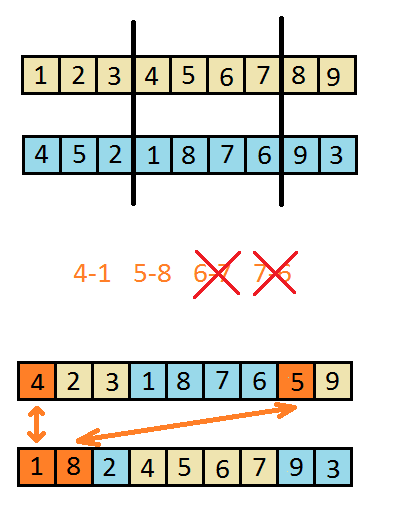
\includegraphics[scale=0.7]{pmx}
\caption{Krzyżowanie PMX}
\end{center}
\end{figure}

Podczas działania operatora OX, czyli operatora z zachowaniem porządku, wybierane są dwie pozycje genów z rozwiązań rodziców i spomiędzy tych pozycji kopiowane są geny z rodzica pierwszego do potomka pierwszego i z rodzica drugiego do potomka drugiego. Następnie, począwszy od pierwszej pozycji za kopiowanym fragmentem, przenoszone są geny z rodzica pierwszego do rozwiązania potomnego nr 2, z wyłączeniem elementów już się w nim znajdujących i na odwrót, czyli geny rodzica drugiego przenoszone są do potomka pierwszego. Przeniesione elementy są również umieszczane od pierwszej pozycji za skopiowanym fragmentem. Poniżej znajduje się rysunek obrazujący działanie tego operatora:

\newpage
\begin{figure}[h]
\begin{center}
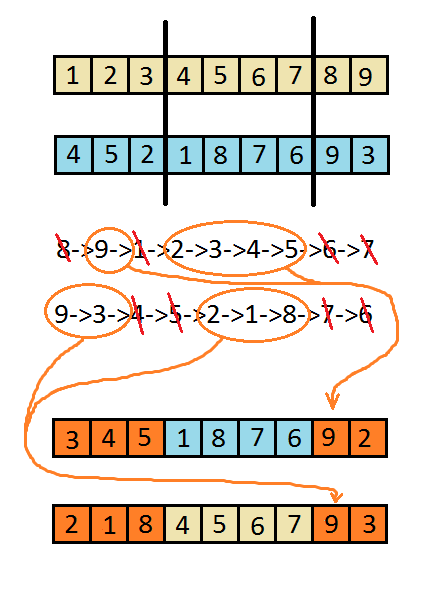
\includegraphics[scale=0.7]{ox}
\caption{Krzyżowanie OX}
\end{center}
\end{figure}

Zgodnie z założeniem autorów algorytmu, prawdopodobieństwo zajścia krzyżowania powinno zmniejszać się wraz z rosnącą liczbą iteracji algorytmu. W zmodyfikowanej wersji algorytmu możliwe jest ustawienie maksymalnego i minimalnego prawdopodobieństwa na tę samą wartość, co skutkuje niezmiennym prawdopodobieństwem krzyżowania podczas działania algorytmu.

Jeśli spośród wybranych na drodze działania operatora selekcji do krzyżowania zostanie przeznaczone mniej rozwiązań niż wynosi rozmiar populacji, z wybranych rozwiązań losowo kopiowane są brakujące osobniki i wstawiane są do listy przeznaczonych do krzyżowania rozwiązań w losowe miejsca. Następnie każde dwa kolejne rozwiązania na liście rodziców poddawane są wybranemu sposobowi krzyżowania i w ten sposób otrzymywane jest następne pokolenie rozwiązań, zastępujące poprzednie.

\subsection{Operator bramki kwantowej}
Oprócz przedstawionych wartości w tabeli \ref{LUT_TAB} zaproponowana została druga wersja tablicy \textit{Look Up}. Kąt zmieniany jest tylko w przypadku, gdy stany porównywanych kubitów są różne. W przypadku, gdy dopasowanie zapamiętanego rozwiązania najlepszego jest mniejsze niż poddawanego działaniu bramki kwantowej, zmiana kąta powoduje zwiększenie prawdopodobieństwa, że dany kubit pozostanie w swoim aktualnym stanie i wartość, o którą zmieniany jest kąt jest stosunkowo mała. W sytuacji, gdy dopasowanie rozwiązania najlepszego jest rzeczywiście lepsze, zmiana kąta następuje w kierunku zwiększenia prawdopodobieństwa, że kubit znajdzie się w stanie takim samym jak porównywany z nim odpowiadający mu kubit z rozwiązania najlepszego. W tym przypadku kąt jest zmieniany o wartość dużo większą niż w poprzedniej sytuacji. Zarówno jednak wartości, o które oba kąty są zmieniane, są dużo mniejsze niż wartości, które zostały zaproponowane w tabeli \ref{LUT_TAB}.

Poniżej znajduje się alternatywna wersja tablicy \textit{Look Up}:
\begin{table}[h]
\label{LUT_TAB_MOD}
\begin{tabular}{l l l l l l l l}
\hline
$r_i$ & $b_i$ & $f(r)<f(b)$ & $\Delta\Theta_i \cdot \pi$ & $s(\alpha_i,\beta_i)$ & & & \\
\cline{5-8} 
& & & & $\alpha_i \cdot \beta_i > 0$ & $\alpha_i \cdot \beta_i < 0$ & $\alpha_i = 0$ & $\beta_i = 0$ \\
\hline
0 & 1 & False & $0.08\pi$  & +1 & -1 & 0         & +1 lub -1\\
0 & 1 & True  & $0.001\pi$ & -1 & +1 & +1 lub -1 & 0\\
1 & 0 & False & $0.08\pi$  & -1 & +1 & +1 lub -1 & 0\\
1 & 0 & True  & $0.001\pi$ & +1 & -1 & 0         & +1 lub -1\\
\hline
\end{tabular}
\caption{Alternatywna LUT dla bramki kwantowej}
\end{table} 

W nieuwzględnionych przypadkach nie następuje aktualizacja kąta. Dotyczy to sytuacji, gdy zarówno kubit z rozwiązania najlepszego i aktualnie poddawanego działaniu bramki kwantowej, znajdują się w tym samym stanie, niezależnie od sytuacji, które z rozwiązań jest lepsze.

\subsection{Pozostałe zmiany}
W stosunku do algorytmu w postaci proponowanej w publikacji \cite{NPQGA}, wprowadzone zostały jeszcze dwie zmiany. Pierwszą z nich jest ustawianie wartości prawdopodobieństwa krzyżowania na wartość $P_{c min}$ w przypadku, gdy wyliczana w każdej iteracji jego wartość spadnie poniżej wartości $P_{c min}$. Druga modyfikacja związana jest z dekodowaniem stanów kubitów. Wedle autorów algorytmu, stan kubitu powinien być ustawiony na wartość 1, gdy wylosowany parametr $\eta$ jest mniejszy niż wartość $|\alpha|^2$, co nie jest prawdą, gdyż $|\alpha|^2$ określa prawdopodobieństwo, że kubit znajduje się w stanie 0.